\documentclass[12pt]{article}
\usepackage[margin=1in]{geometry}
\usepackage[T1]{fontenc}
\usepackage{mathptmx}
\usepackage[parfill]{parskip}
%\usepackage{amsmath}
\usepackage{graphicx}
%\usepackage{listings}   % allows lstlisting environment
%\usepackage{moreverb}   % allows listinginput environment
%\usepackage{siunitx}
%\usepackage{enumerate}
%\usepackage{epstopdf}
%\usepackage{booktabs}
%\usepackage{float}
%\usepackage{multirow}
%\usepackage{mhchem}
%\usepackage{lscape}
\usepackage{hyperref}
\hypersetup{
    colorlinks=true,
    linkcolor=blue,
    filecolor=magenta,      
    urlcolor=cyan,
}

\newcommand{\horrule}[1]{\rule{\linewidth}{#1}} % Create horizontal rule command with 1 argument of height

\newcommand\mytitle{Evolution 2\\Compsci 458}
\title{\horrule{5pt}\\\vspace{0.4cm}{\bf \mytitle}\\}
\author{Jiawei Zhang, Davis Treybig, Michael Han, and Kevin Do}
\date{\horrule{1pt}}

\begin{document}
\maketitle{}
\section{Summary}
\begin{figure}[h]
\begin{center}
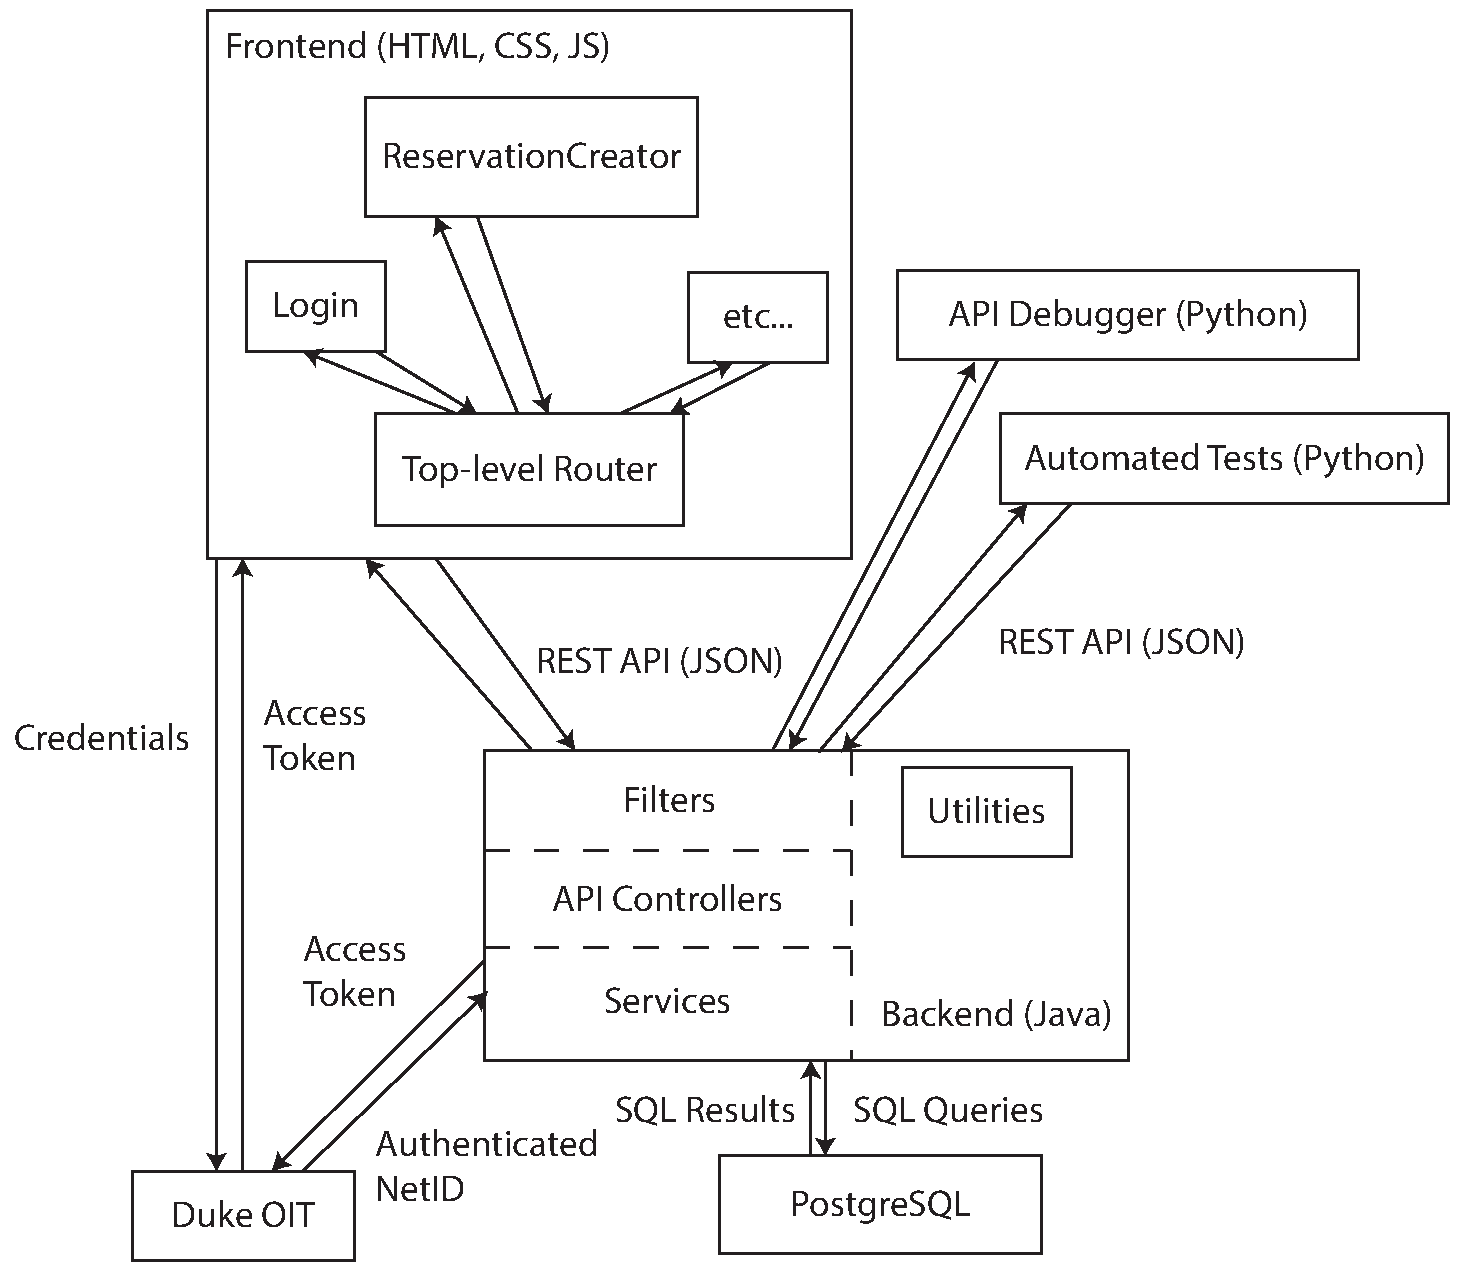
\includegraphics[height=4in]{ev2_design_cropped.pdf}
\end{center}
\caption{Diagram of system architecture}
\label{fig:design}
\end{figure}

Our resource management tool is a web application that uses the following technology stack: a React.js frontend, a Java Spring server, and a PostgreSQL database. In addition, we use Python scripts to automate the testing of our API. Our overall technology stack, as well as our overall code structure, have not changed since evolution 1. As can be seen in the diagram above, the two primary changes are:
\begin{enumerate}
    \item The inclusion of an API Debugger. This is just a python script that interacts with our backend, similarly to the way our python API tests function. 
    \item The inclusion of OAuth2 to handle duke net-id based authentication. TODO: Jiawei briefly explain this
\end{enumerate}

The rest of the changes required for evolution 2 fit nicely into our existing frameworks. In the backend, permissions were handled with a few new API calls on top of our evolution 1 API calls, and a few new DB tables were added to support these calls. Similarly, groups were implemented via the addition of another controller and service. In the frontend, new views for permissions and groups were added.  

For retrospectives on our former backend choices and more detail about our backend additions, see the \hyperref[sec:Backend]{backend section}. For retrospectives on our former frontend choices and more detail about our frontend additions, see the \hyperref[sec:Frontend]{frontend section}. Finally, see \hyperref[appendix:backendtest]{Appendix \ref{appendix:backendtest}} for our updated backend test strategy,  \hyperref[appendix:frontendtest]{Appendix \ref{appendix:frontendtest}} for our updated frontend test strategy, \hyperref[appendix:apispec]{Appendix \ref{appendix:apispec}} for our updated API specification, and \hyperref[appendix:DBDesign]{Appendix \ref{appendix:DBDesign}} for our updated database design. 

\section{Backend}
\label{sec:Backend}
TODO rewrite?

The backend consists of the parts of the software system that run on a VPS (Virtual Private Server) using Ubuntu Linux 14.04. Our software uses PostgreSQL 9.5 for persistent data storage and the Java Spring Framework as the container for a Tomcat web server. If the backend were viewed as an MVC (Model-View-Controller), PostgreSQL would be the model and Java Spring would be the view (REST API) and the controller (request processing, database communication, and response creation). 

\subsection{Java}
\subsubsection{Retrospective}
TODO
\subsubsection{Current Design}
TODO

The majority of the backend is written in Java. We chose Java for a few key reasons:
\begin{enumerate}
    \item It is statically typed. A common class of bugs is caused by an interface mismatch between two pieces of code. Static typing can help enforce interfaces and therefore prevent these types of bugs.
    \item We found Spring (our Java server framework) to be easy to use and simple to understand, with a huge amount of documentation and support. It is also very powerful and used in many enterprise applications. 
    \item Our whole team is intimately familiar with Java. 
    \item Java has good cross-platform support across all potential server operating systems offered by Duke OIT's VM service. By contrast, we were not confident in Ubuntu's C\# support through the Mono runtime. Java also has a large standard library and many community libraries, further easing the development process. 
\end{enumerate}

\subsection{Java Spring}
\subsubsection{Retrospective}
TODO
\subsubsection{Current Design}
TODO

There are a number of open-source application frameworks for Java. Some of the prominent ones that our team looked into are \href{https://www.playframework.com/}{Play}, \href{https://jax-rs-spec.java.net/}{JAX-RS}, \href{http://sparkjava.com}{Spark}, and \href{https://spring.io/}{Spring}. Ultimately, we chose to use Spring, for the following reasons:
\begin{enumerate}
    \item Spring is the oldest, most mature Java web framework. It thus has fantastic documentation and support, as well as a large number of supporting libraries.  These factors make Spring easy to learn, which is vital in the context of a class project where we have to get started developing right away. 
    \item The most common criticism of Spring is that it is too heavy-duty for simple applications. We built a sample application to evaluate this criticism and decided it was overstated.
\end{enumerate}

\subsection{PostgreSQL}
\subsubsection{Retrospective}
TODO
\subsubsection{Current Design}
TODO

PostgreSQL is an open-source object-relational database management system. 

We chose Postgres over other free, open-source relational databases like MySQL because we were familiar with it. Furthermore, we were swayed by PostgreSQL's focus on compliance and predictability, which was more important to us than MySQL's raw performance.

We chose PostgreSQL over non-relational databases (e.g. MongoDB, Cassandra, CouchDB) because we wanted our data to be structured, which, like static typing, helps reduce bugs. One drawback to relational databases is that costly and complicated database migrations may need to be run when making changes to the database schema. However, given that we don't need to persist data across evolutions, this drawback is moot.

In designing the DB schema, we did not attempt to prematurely guess what changes might be made to the requirements in the future (for instance, it is conceivable that in the future a reservation could have multiple resources, which would alter the schema quite a lot). We felt like trying to do so would add a lot of work, but potentially offer minimal reward, particularly if we guessed incorrectly. As such, we instead focused on creating a simple schema that would appropriately handle the current set of requirements.


\subsection{Security}
\subsubsection{Retrospective}
TODO
\subsubsection{Current Design}
TODO

The application has multiple layers of protection. When a user is created by the admin, a random salt is generated and appended to the password, which is then SHA-1 hashed. Upon login, the salt is appended to the entered password, hashed, and compared to the stored hash. 

Upon login, a JSON Web Token (JWT) is generated, which stores the User ID and permission level of the logged-in user. This JWT, which is signed by a secret key known only to the server, authenticates future API calls without accessing the database. Instead of a database lookup, the authenticity of the JWT is confirmed using the secret key, and the User ID and permission level stored in the JWT can be used directly. 

For encrypting the communication between the client and the server, we decided to go with SSL as Spring provided support for it. We used Java's built in keytool to generate a Java keystore and self-signed certificate using RSA algorithm. We used a self-signed certificate rather than one signed by a legitimate CA because it was free. We also made it so that it can run on both HTTP and HTTPS at the same time for ease of testing. Non-SSL HTTP support can easily be disabled with a global switch.

\subsection{Testing}
\subsubsection{Retrospective}
TODO
\subsubsection{Current Design}
TODO

For backend testing, we wrote automated tests using Python (\hyperref[appendix:backendtest]{Appendix \ref{appendix:backendtest}}). We chose not to use Spring's built-in testing because it is exceptionally difficult to get working correctly. In contrast, Python scripts are easy to run, simple to understand, and easy to rapidly update and add more tests to. Python's testing framework \texttt{unittest} also has a test discovery function which runs every test with ``test'' in the function name. This feature means that we do not have to manually update a separate testing script whenever we add a new test, thus improving our design.

Our testing script currently tests only the API contract, and not any internals of the backend. This choice is for two reasons. First, the API contract is ultimately the layer that must be working for our front-end application to work, and thus if it works, it is highly likely that there are no significant issues or bugs in our backend code. To some extent, if the application is working from the perspective of the end-user, then it is working correctly. Secondly, it is much harder to test the internals of the back-end, mostly because of our issues using Spring's testing paradigm. That being said, it may be in our best interest to add unit tests in the future if we can figure out how. 

We spent the time to create and maintain an automated testing script because it helps us identify newly introduced bugs much more quickly, and gives each member of the team assurance that they can quickly make changes to the backend without having to manually test after every change. This assurance speeds up our development cycle. In addition, because automated tests perform the same steps every time, the expected results are consistent which is not always the case with manual testing.

\subsection{Code Structure}
\subsubsection{Retrospective}
TODO
\subsubsection{Current Design}
TODO

Our backend code is primarily divided into Filters, Controllers, Services, and Utilities. These components have the following responsibilities: 
\begin{enumerate}
    \item Filters act upon nearly all incoming requests. For instance, we must verify that most API requests contain an appropriate authorization token. 
    \item Requests are then routed to the appropriate method in the appropriate Controller based on the request's URL.
    \item Services handle the actual logic of each request, interacting with the database as needed. 
    \item Finally, each Service may call on one or more Utility classes, which contain common functionality used across multiple services, such as converting time data structures or hashing passwords. 
\end{enumerate}

The above structure allows our backend to be flexible in the face of requirement changes. Because we separate out request filtering (Filters), request routing (Controllers), request logic (Services), and common functionalities used across multiple request types (Utilities), we are easily able to add new filters, add or change API endpoints, or modify our backend logic for individual requests without having to change multiple classes or methods. 

\section{REST API}
\label{sec:REST}
Communication between the frontend and the backend is done through a REST API with JSON (\hyperref[appendix:apispec]{Appendix \ref{appendix:apispec}}).

\subsection{Retrospective}
The JSON-based REST API served us well for Evolution 2. We identified several strengths that helped us implement the new set of requirements: the well-understood nature of JSON and the fairly rich state transfer afforded to us. Furthermore, the weaknesses we identified (that the client must initiate all data transfer and JSON's rigid tree-of-values structure) did not affect us much when implemented Evolution 2.

One unexpected strength of our REST API was the requirement in Evolution 2 of having an API. In the early stages of the project, we were debating between server-side rendering and client-side rendering. Server-side rendering (e.g. Ruby on Rails) involves the server performing virtually all of the business logic and sending to the client fairly static HTML pages. Each time the user performs an action, he/she is taken to a new page that is rendered from scratch. By contrast, client-side rendering sees the user download a client application, which then executes API calls against the backend and updates the view. We chose to implement client-side rendering because it enables quicker UI updates (because typical REST API payloads are much smaller than typical webpages), but we did not anticipate the additional benefit that having a well-defined API meant that we could externalize the API when Evolution 2 asked us to.

\subsection{Current Design}
We expanded the set of endpoints that were required to implement the requirements in Evolution 2. Endpoints for creating, updating, and deleting groups were virtually identical to endpoints we had already written, so completing the groups feature went quickly. Endpoints for updating permissions was also similar to previous work. The slightly more complicated endpoints were those involved in OAuth authentication. Even then, the complexity was inherent to any OAuth implementation and we were not hindered by our previous design choice of a RESTful JSON API.

\section{Frontend}
\label{sec:Frontend}
The frontend consists of the parts of the software system that are transferred to the user's computer and are run in the user's browser. The officially supported browser is the latest version of Google Chrome, but other modern browsers should work as well. We use the third-party libraries React.js, Bootstrap, and JQuery, but React.js has the most implications for the code design.

\subsection{React.js}
\subsubsection{Retrospective}
The frontend is written in React.js, a library written at Facebook for building user interfaces (UIs). We have been pleased with React.js. Our only complaint has been that React.js has occasionally required somewhat large amounts of boilerplate. We have read online that this boilerplate can be significantly reduced with some more advanced React.js techniques like mix-ins. We plan to take advantage of this in future React.js projects, but for now the cost of updating the code to use mix-ins would be higher than the benefit of more concise code.

As we discussed in our Evolution 1 writeup, using React.js allows us to trivially avoid inconsistent UIs, since the view is re-rendered from the whole state. As expected, we did not encounter a single UI bug due displaying inconsistent data.

\subsubsection{Current Design}
We made no changes to our usage of React.js, as we were quite pleased with it.

\subsection{React components}
\subsubsection{Retrospective}
Within the React framework, we designed components to express the desired UI in a natural way. At the top level of the HTML body is a Router component. This Router's state includes a route and other state to mediate communication between views. The route is a string that indicates which part of the application the user is in (e.g. ``reservation\_list'').

The Router, depending on its route state, will render another component (e.g. Login, AdminConsole, ReservationList, GroupManager). All of these views are themselves just HTML renderings of their state. Each of these subcomponents contains their own state. We considered having a global datastore of resources and reservations, but decided that the simplest way to maintain correctness across views was to simply redownload the data each time.

This design served us well. One minor issue we encountered was related to sending information between components. Because the components rendered by the Router do not have knowledge about eachother, they must send information through the Router, which then passes the information as a 'prop' to the receiving subcomponent . Though this has worked well in practice, it does seem a bit unwieldy.

\subsubsection{Current Design}
For the new requirements in Evolution 2, we added a GroupManager component and a PermissionsManager component. We also made minor modifications to some of the other components built for Evolution 1. Because the components were completely separate, this task did not take long and we did not encounter any unexpected challenges. We are therefore quite pleased with our design, since it appears to conform to the open-closed principle.

\subsection{Testing}
\subsubsection{Retrospective}
For frontend testing, we decided to write a test plan (\hyperref[appendix:frontendtest]{Appendix \ref{appendix:frontendtest}}) that is intended to be performed manually. Testers can load the application and execute actions that are intended to exercise most of the code paths in the application. This manual testing has the advantage that it has a low upfront cost and it is easy to implement. The disadvantage is that it is slow and takes a lot of human time and energy.

One alternative is to perform automated UI testing. We are aware of two different types automated UI testing: 1) programmatic access to the application and 2) simulation of mouse/keyboard events and screenshots. We decided against 1) because the UI is still in an infantile stage, and the intended DOM changes quite frequently. We decided that programmatically testing for the presence of, say, a certain <div> tag would be prohibitively expensive. We decided against 2) for the same reason that the intended DOM changes quite frequently, but also because we decided that such an approach seemed very fragile.

We were very pleased with our decision not to implement automated UI testing. While we did encounter some UI bugs, these bugs did not take long enough to catch that they would have justified the significant cost of implementing automated UI testing. (It's important to note that automated UI testing only decreases the amount of time it takes to catch bugs, not the amount of time it takes to fix them, a process which is more properly called \emph{debugging}.)

\subsubsection{Current Design}
As a result of our success with the manual UI testing from evolution 1, the only changes to our methodology here are to increase the number of test cases to account for the new functionality introduced by the Evolution 2 requirements (TODO add testcases to appendix).

\section{Member contributions}
Kevin Do maintained the frontend, advocated for the frontend's needs in discussions with the backend team, and implemented the permissions manager.

Davis Treybig implemented much of the permission-related code, including new permission endpoints and permission-based checks for other API endpoints. 

Jiawei Zhang implemented the OAuth system and the group management endpoints and TODO.

Michael Han wrote and maintained the automated backend tests, and he also implemented the group manager UI TODO.

\clearpage
\appendix
\section{Backend Test Plan}
\label{appendix:backendtest}
\begin{enumerate}
	\item Authorization Tests
	\begin{enumerate}
		\item Registering a valid user
		\item Registering an invalid user with preexisting email
		\item Registering an invalid user without a password
		\item Logging in as valid user
		\item Logging in with wrong password
		\item Logging in with wrong email, correct username and password
		\item Logging in with wrong username, correct email and password
	\end{enumerate}
	\item Resource Tests
	\begin{enumerate}
		\item Create valid resource with no tags
		\item Create valid resource with tags
		\item Create invalid resource with no name
		\item Create valid resource with no description 
		\item Get resource with valid ID
		\item Get resource with invalid ID
		\item Get resources with valid query
		\item Get resources with query with non existing tags
		\item Put resource with valid ID with all fields updated
		\item Put resource with valid ID no fields updated
		\item Put resource with invalid ID
		\item Delete resource with valid ID
		\item Delete resource with invalid ID
		\item Get resources canDelete with valid ID
		\item Get resources canDelete with invalid ID
	\end{enumerate}
	\item Reservation Tests
	\begin{enumerate}
		\item Create valid reservation with valid user ID
		\item Create valid reservation with invalid user ID
		\item Create reservation with touching time intervals
		\item Create invalid reservation with invalid resource ID
		\item Create invalid reservation with invalid time range
		\item Get reservation with valid ID
		\item Get reservation with invalid ID
		\item Get reservation with valid query with resource and user lists
		\item Get reservation with valid query with valid time range
		\item Get reservation with valid query with invalid time range
		\item Put reservation with valid ID update all fields
		\item Put reservation with valid ID update no fields
		\item Put reservation with invalid ID
		\item Delete reservation with valid ID
		\item Delete reservation with invalid ID
	\end{enumerate}
	\item Tags Tests
	\begin{enumerate}
		\item Get all tags
	\end{enumerate}
	\item User Tests
	\begin{enumerate}
		\item Check only admin can create users
		\item Check that non admin cannot create users
		\item Create invalid user with preexisting username
		\item Create invalid user with preexisting email 
		\item Get user with valid ID
		\item Get user with invalid ID
		\item Put User with invalid ID
		\item Put user not as admin
		\item Delete user with valid ID
		\item Delete user with invalid ID
	\end{enumerate}
\end{enumerate}

\clearpage
\section{Frontend Test Plan}
\label{appendix:frontendtest}
\begin{enumerate}
	\item Login
	\begin{enumerate}
		\item Logging in as the admin works
		\item Logging in as a normal user works
		\item Entering the wrong credentials -> useful message
	\end{enumerate}
	\item Navbar
	\begin{enumerate}
		\item Resources -> resources list
		\item Reservations -> reservations list
		\item Admin console works
		\item Log out works
	\end{enumerate}
	\item Reservations List
	\begin{enumerate}
		\item Start+end can correctly filter reservations shown
		\item Tags can correctly filter reservations shown
		\item Can properly go to the ``New reservation'' view
		\item Can properly go to the ``Edit reservation'' view
		\item Normal user can delete reservations own reservations
		\item Normal user can NOT delete others' reservations
		\item Admin can delete any reservation
	\end{enumerate}
	\item Resources list
	\begin{enumerate}
		\item Tags can correctly filter resources shown
		\item Can properly go to the ``New resource'' view
		\item Normal user can not edit/delete anything
		\item Admin user can edit/delete anything
		\item Deleting a resource with a future reservation shows a warning
	\end{enumerate}
	\item New resource
	\begin{enumerate}
		\item Admin can make new resource
		\item Normal user can't make new resource
		\item Displays error messages when invalid
	\end{enumerate}
	\item New reservation
	\begin{enumerate}
		\item Normal user can make new reservation with their own user ID
		\item Normal user can't make new reservation with another user ID
		\item admin can make new reservation with any user ID
	\end{enumerate}
	\item Admin console
	\begin{enumerate}
		\item Admin can make new user
		\item Normal user can't make new user
	\end{enumerate}
\end{enumerate}

\clearpage
\section{API Specification}
\label{appendix:apispec}
\begin{enumerate}
\item POST /auth/register
Creates an account with specified email and password

Common errors: email taken

Returns a JSON object with is\_error (boolean), error\_msg (possibly empty string)

\item POST /auth/login
Logs into an account with specified email and password

Common errors: invalid email or password

Returns a JSON object with is\_error (boolean), error\_msg (possibly empty string). If is\_error is false, also returns the session token


\item POST /resources
Creates a resource with the specified name, description, and tags, and assigns it a new unique ID

Common errors: empty name

Returns a JSON object with is\_error (boolean), error\_msg (possibly empty string). If is\_error is false, also returns a resource subobject with all the fields that were actually committed (ideally, the same as the values that were passed in)

\item GET /resources/<ID>
Returns a JSON object with is\_error (boolean) and error\_msg (possibly empty string)

Common errors: Resource with the specified ID does not exist

If is\_error is false, also returns a ``resource'' subobject with all the fields of the resource with the supplied ID

\item GET /resources/
Runs the specified query on the set of all resources and returns those that match

Queries are specified by a URL parameters with a ``required\_tags'' object (list of strings) and ``excluded\_tags'' specifying the tags that the resources in the search results should all have

Returns a JSON object with is\_error (boolean) and error\_msg (possibly empty string)

If is\_error is false, also returns a ``resources'' subobject, a list of resources (including ID and all fields) that match the query

\item PUT /resources/<ID>
Updates a resource with the supplied ID. Only changes the supplied fields and leaves the rest alone

Returns a JSON object with is\_error (boolean), error\_msg (possibly empty string). If is\_error is false, also returns a resource subobject with all the fields that were actually committed (ideally, the same as the values that were passed in)

\item DELETE /resources/<ID>
Deletes the resource with the given ID, if it exists, AND deletes all associated reservations

Common error: resource with the specified ID does not exist

Returns a JSON object with is\_error (boolean) and error\_msg (possibly empty string)

\item POST /reservations
Creates a reservation with data specified by the payload's ``resource\_id'' (int), ``start\_timestamp'' (string), ``user\_id'' (int), and ``end\_timestamp'' (string), ``should\_email'' (boolean) fields and assigns it a new unique ID

Validates the user ID for the reservation based on the currently authenticated user

Returns a JSON object with is\_error (boolean), error\_msg (possibly empty string). If is\_error is false, also returns a reservation subobject with all the fields that were actually committed (ideally, the same as the values that were passed in)

\item GET /reservations/<ID>
Returns a JSON object with is\_error (boolean) and error\_msg (possibly empty string)

If is\_error is false, also returns a ``reservation'' subobject with all the fields of the resource with the supplied ID

\item GET /reservations/
Runs the specified query on the set of all reservations and returns those that match

Queries are specified by URL parameters with one or more of the following: ``resource\_ids'' field (list of ints) specifying the desired resource IDs of the reservations (ANY), ``user\_ids'' (list of ints) (ANY), ``start'' (string, ISO 8601), ``end'' (string, ISO 8601)

return anything that overlaps with time range. If no user\_ids or resource\_ids are specified, return ALL reservations in time range. 

Returns a JSON object with is\_error (boolean) and error\_msg (possibly empty string)

If is\_error is false, also returns a ``reservations'' subobject (list of objects), a list of reservations (including ID and all fields) that match the query, ``resources'' subobjects (list of resource objects used in reservations), and ``users'' subobject (list of users objects used in reservations)

\item PUT /reservations/<ID>
Updates a reservation with the supplied ID. Only changes the supplied fields and leaves the rest alone

Returns a JSON object with is\_error (boolean), error\_msg (possibly empty string). If is\_error is false, also returns a reservation subobject with all the fields that were actually committed (ideally, the same as the values that were passed in)

\item DELETE /reservations/<ID>
Deletes the reservation with the given ID, if it exists

Common error: no reservation with specified ID

Returns a JSON object with is\_error (boolean) and error\_msg (possibly empty string)


\item GET /tags
Returns a JSON object with ``tags'' (list of strings), a list of all tags

\item GET /resources/<ID>/canDelete
Returns whether future/current reservations exist relating to a resource, in order to see whether we want to delete. This should return true if and only if (any reservations overlap the current time or start after the current time).

Returns a JSON object with is\_error (boolean), error\_msg (possibly empty string). If is\_error is false, also returns a boolean ``can\_delete'' with the answer

\item POST /users
Creates a given user with data specified by the payload's ``email'' (string), ``password'' (string), ``username'' (string), ``should\_email'' (bool), A unique ID is automatically assigned by the DB. 

Error cases: must check that no user already exists with the given username. Must also verify that the admin is the one doing this (only admin can create users)

Returns a JSON object with is\_error (boolean), error\_msg (possibly empty string). If is\_error is false, also returns the user subobject that was created

\item GET /users/<ID>
Retrieves the user with a given ID, if such a user exists. 

Returns a JSON object with is\_error (boolean), error\_msg (possibly empty string). If is\_error is false, also returns the user subobject. 

\item PUT /users/<ID>
Updates a user with the supplied ID. Only changes the supplied fields and leaves the rest alone

Error Check: If username changes, must verify the new username is not already taken. Must also verify that the admin is the one doing this (only admin can modify users)

Returns a JSON object with is\_error (boolean), error\_msg (possibly empty string). If is\_error is false, also returns the full, updated user subobject. 

\item DELETE /users/<ID>
Deletes the user with the supplied ID. 

Error Check: verify that the user with the given ID exists

Returns a JSON object with is\_error (boolean) and error\_msg (possibly empty string)
\end{enumerate}

\clearpage
\section{DB Design}
{\huge TODO}
\label{appendix:DBDesign}


\end{document}